\chapter{Verification and code audit}\label{ch:c8}\label{ch:verification}
This chapter reports how the coupling was tested and what was found. Nine complementary approaches were used
(Table~\ref{tab:vapproach}); every problem they uncovered is listed, with its correction, in Section~\ref{sec:findings}.

\begin{plain}
Before anyone relies on a model, it must be shown to be right. The coupling was tested in several independent ways:
automatic checks that no water is created or lost, comparisons with exact textbook solutions, comparisons with independent
software, hundreds of random test set-ups, and a line-by-line review of the code. Every problem found along the way is
listed at the end of the chapter with how it was fixed.
\end{plain}

\begin{table}[!htbp]\centering
\caption{Verification approaches.}\label{tab:vapproach}
\begin{tabularx}{\linewidth}{P{0.27\linewidth}Y P{0.13\linewidth}}\toprule\hdr
Approach & What it shows & Section\\\midrule
Regression against Raven 4.15 & models without groundwater give identical results & \ref{sec:regression}\\
Automated audit of every run & exact water accounting on both sides; MODFLOW's balance & \ref{sec:audit}\\
Behaviour tests & pumping, drying, restarts, ensembles and every exchange behave as expected & \ref{sec:behaviour}\\
Grid types & geometry, format cross-checks, analytical solution, restarts and randomized tests for every grid & \ref{sec:vgrids}\\
Existing model & projections, units, round trip, overlap weights, restarts, safeguards, randomized tests & \ref{sec:vexisting}\\
Independent checks & geometry against standard libraries; flows against MODFLOW's own budget; grid and time-step invariance; faulty input & \ref{sec:independent}\\
Randomized testing & hundreds of random set-ups combining every option & \ref{sec:fuzz}\\
Release audit & five-step audit of the final package; checks of every MODFLOW input file and of faulty input without MODFLOW; one command repeats every test & \ref{sec:relaudit}\\
Code audit & line-by-line review, compiler, static analysis, memory and undefined-behaviour sanitizers & \ref{sec:codeaudit}\\\bottomrule
\end{tabularx}
\end{table}

\section{Models without groundwater are unchanged}\label{sec:regression}
The coupling was developed on Raven~4.1.1 and then carried over to Raven~4.15 (Section~\ref{sec:port}). Models without
groundwater were run with the unmodified Raven~4.15 and with the coupled code, both built with NetCDF:
\begin{itemize}
\item the Liard model: all outputs identical byte for byte;
\item the benchmark models distributed with Raven (\cmd{benchmarking/\_InputFiles}): the eleven that run give identical
      outputs, except that Lake of the Woods, whose reservoir in basin~44 dries out on 45 days, books less evaporation on
      those days (the correction of Section~\ref{sec:findings}). Its hydrographs and reservoir stages are identical; its
      cumulative balance error falls from 5.44 to 4.97~mm, and its \cmd{solution.rvc} carries the reservoir stages with 12
      digits. The other fourteen benchmark set-ups stop with the same input error in both builds (a missing \cmd{.rvt} file,
      wilting point above field capacity), as they do in the unmodified Raven~4.15.
\end{itemize}
The corrections made to Raven itself (Section~\ref{sec:findings}) affect only ensembles, reservoirs with absolute stages or
that dry out, restart files, constituent observations and the \cmd{:rvg\_Filename} command.

\subsection{Carrying the coupling over to Raven 4.15}\label{sec:port}
Between 4.1.1 and 4.15, 157 of Raven's source files changed. A three-way merge (Raven~4.1.1, the coupling, Raven~4.15) left 26
overlapping edits in 22 files; each was resolved by hand:
\begin{itemize}
\item copyright headers (13): the 4.15 year kept, with the line naming the modification;
\item observation diagnostics: 4.15's new rule for observations without a subbasin kept, with \cmd{GW\_HEAD} handled
      first (its location is a monitoring well);
\item initial conditions: the new groundwater commands of the \cmd{.rvc} file beside 4.15's new management commands;
\item ensembles: 4.15's \cmd{RebootTimeVariables} (which resets the balance arrays between members) kept beside the
      restoring of routing memory and reservoir states; the history setters now take the time step, as in 4.15;
\item reservoirs: 4.15 replaced the data-assimilation scale factor by an additive adjustment; the reservoir snapshot for
      ensemble members and the 12-digit \cmd{solution.rvc} values follow that change;
\item BMI: 4.15 had already corrected the index in \cmd{SetValueAtIndices} in the same way, so its version was taken;
\item the Visual Studio project files were rebuilt from 4.15's, with the MODFLOW-USG files replaced by the new ones.
\end{itemize}
Raven~4.15 prints its closing message (\emph{Exiting Gracefully}) to the error stream; the test scripts read both streams.
The whole test suite was then repeated on the ported code with MODFLOW~6.8.1 and~6.6.3 (Section~\ref{sec:relaudit}).

\section{Automated audit of every run}\label{sec:audit}
The tool \cmd{tools\_audit.py}, shipped with the example, checks any output folder for:
\begin{enumerate}
\item \textbf{recharge:} $\left(\sum V^{\mathrm{Raven}}-\sum V^{\mathrm{MF6}}-\Delta S^{\mathrm{delay}}-\sum V^{\mathrm{CHD}}\right)/\sum V^{\mathrm{Raven}}$;
\item \textbf{MODFLOW's balance:} cumulative imbalance relative to the gross flow, and the worst single step;
\item \textbf{convergence:} steps that failed to converge;
\item \textbf{seepage, rivers and surface stores:} the volume applied to Raven against MODFLOW's flow, including carried river losses;
\item \textbf{reservoirs:} the seepage sent to MODFLOW each step against the volume that left the lake the step before, and
      the volume MODFLOW took against the volume sent;
\item \textbf{Raven's balance:} the largest mass-balance error in \cmd{Watershed\allowbreak Storage.csv};
\item \textbf{outputs:} finite heads, contiguous end-of-step dates, a $t=0$ row for monitoring wells.
\end{enumerate}
Table~\ref{tab:audit} gives the results. They were first obtained before the release audit (Section~\ref{sec:relaudit}); with
the final code the 20-year Liard run gives outputs identical to those runs, and the reservoir and ensemble runs were repeated
(Section~\ref{sec:behaviour}).

\begin{table}[!htbp]\centering
\caption{Automated audit (\cmd{tools\_audit.py}); the reservoir and ensemble rows are from the final code's repeat (\cmd{tests/behaviour\_check.py}), the 20-year Liard run is identical with the final code. Relative errors are shares of the water moved. In every run the seepage returned to Raven equals MODFLOW\textquotesingle s seepage exactly, the surface-store bookkeeping is exact, no river loss is carried at the end and the output dates are contiguous. The one failed step is the rewetting day of the deliberately extreme drying test (Section~\ref{sec:behaviour}).}\label{tab:audit}
\footnotesize\setlength{\tabcolsep}{2.8pt}\begin{tabular}{lrrrrrrr}\toprule\hdr
Run & Steps & Recharge & \shortstack[r]{MODFLOW\\residual} & \shortstack[r]{Worst\\step [\%]} & \shortstack[r]{Failed\\steps} & River & \shortstack[r]{Raven\\balance [mm]}\\\midrule
20-year Liard & 7\,305 & 0 & $-1.0\times10^{-10}$ & $4.2\times10^{-6}$ & 0 & $1.1\times10^{-12}$ & 0.52\\
Pumping & 1\,826 & 0 & $-1.6\times10^{-10}$ & $7.1\times10^{-6}$ & 0 & $-9.6\times10^{-12}$ & 0.52\\
Fixed head, delay & 730 & $-3.2\times10^{-11}$ & $-3.9\times10^{-10}$ & $5.1\times10^{-6}$ & 0 & $7.7\times10^{-12}$ & 0.52\\
Restart & 365 & $-1.7\times10^{-11}$ & $-1.9\times10^{-10}$ & $3.2\times10^{-6}$ & 0 & $2.1\times10^{-11}$ & 0.06\\
Ensemble & 731 & 0 & $-1.7\times10^{-11}$ & $1.6\times10^{-7}$ & 0 & $9.5\times10^{-12}$ & 0.52\\
Wetlands & 730 & 0 & $-1.1\times10^{-10}$ & $1.5\times10^{-6}$ & 0 & $2.2\times10^{-11}$ & 0.52\\
Reservoir & 731 & 0 & $-1.7\times10^{-11}$ & $1.6\times10^{-7}$ & 0 & $9.5\times10^{-12}$ & 0.52\\
Soil-less HRUs & 365 & 0 & $-4.5\times10^{-11}$ & $7.4\times10^{-7}$ & 0 & $-1.2\times10^{-12}$ & 0.52\\
Drying (extreme) & 1\,826 & 0 & $-3.1\times10^{-4}$ & 43.2 & 1 & $8.1\times10^{-12}$ & 0.52\\
\bottomrule\end{tabular}\end{table}


\section{Behaviour tests}\label{sec:behaviour}
\begin{table}[!htbp]\centering
\caption{Behaviour tests.}\label{tab:behaviour}
\begin{tabularx}{\linewidth}{P{0.19\linewidth}P{0.27\linewidth}Y}\toprule\hdr
Test & Set-up & Result\\\midrule
Full Liard model & 20 years, 85 coupled HRUs, 3\,252 active columns & recharge exact; MODFLOW residual $10^{-10}$; no failed step; Raven balance 0.52 mm\\
Pumping & 100\,000 m$^3$/d well, 5 years & 93\% delivered; seasonal drawdown 0.8--8 m in the pumped cell, none 12 km away; 91--98\% of the water captured from rivers (Figure~\ref{fig:pumping})\\
Monitoring wells & synthetic heads with 5 cm noise & RMSE 4.9 cm; NSE 0.991--0.9997\\
Fixed-head lake & 9 cells & heads held exactly; recharge on them redistributed\\
Restart & 1 + 1 years against 2 years & flows within $6\times10^{-6}$ (Figure~\ref{fig:hotstart})\\
Ensembles & 2 Monte Carlo members, every option on & members identical to each other and to a single run\\
Drying and rewetting & valley aquifer starting dry & 26 wet areas merge into 2 and split with the seasons (Figure~\ref{fig:conn}); one rewetting step of 1\,826 does not converge and is flagged\\
Wetlands and lakes & 1\,903 exchange cells & water removed from Raven equals MODFLOW's leakage exactly\\
Reservoir & 50 km$^2$ lake on a coupled HRU & seepage delivered each day equals Raven's seepage of the day before\\
Soil-less HRUs & glacier HRUs coupled & seepage goes to surface water; balance unchanged\\
Other features & \cmd{:rvg\_Filename}, NetCDF, linkage cache, calibration & file found; NetCDF equals the binary heads within $10^{-4}$ m; cached run identical; DDS recovers gravel $K$ and $S_y$ within 5\%\\\bottomrule
\end{tabularx}
\end{table}

The tests on the regular-grid Liard model were first run before the release audit. With the final code (MODFLOW 6.8.1) the
20-year run gives outputs identical to that earlier run --- budget, heads, hydrographs, storage and restart file --- so these
results and the figures drawn from them stand. The two rows the audit's corrections could change were repeated with the final
code (\cmd{tests/behaviour\_check.py}): a 50~km$^2$ lake with seepage on the largest coupled HRU of subbasin~52, with a
pumping well, for two years --- the seepage MODFLOW received each day equals the volume that left the lake the day before
(difference 0), all of it delivered, MODFLOW residual $1.7\times10^{-11}$; and the same set-up as a two-member ensemble ---
both members identical to the single run (difference 0).

\begin{figure}[!htbp]\centering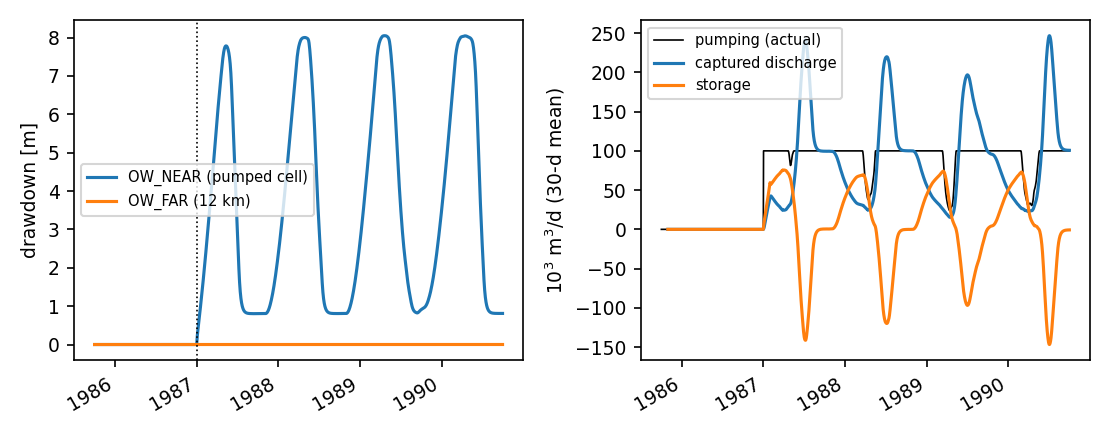
\includegraphics[width=\linewidth]{figures/fig_pumping.png}
\caption{Pumping test: drawdown at the monitoring wells (left) and where the pumped water comes from (right).}\label{fig:pumping}\end{figure}
\begin{figure}[!htbp]\centering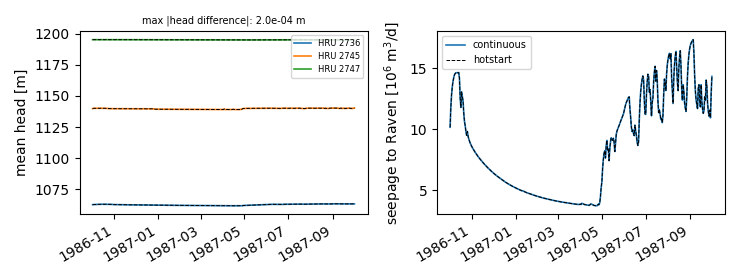
\includegraphics[width=\linewidth]{figures/fig_hotstart.png}
\caption{Restart: the second year of a continuous run (solid) and of a run restarted from \cmd{solution.rvc} (dashed).}\label{fig:hotstart}\end{figure}
\begin{figure}[!htbp]\centering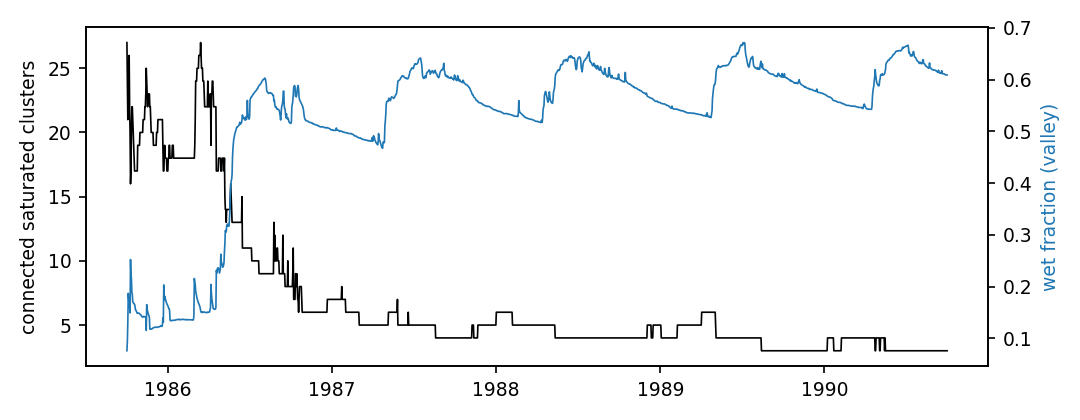
\includegraphics[width=0.9\linewidth]{figures/fig_connectivity.png}
\caption{Drying and rewetting: number of separate wet areas in the top layer (black) and wet fraction of the valley aquifer (blue).}\label{fig:conn}\end{figure}

\section{Independent checks}\label{sec:independent}
\subsection{Geometry against standard libraries}
The geometry functions were compiled into a stand-alone test and compared with widely used libraries (Table~\ref{tab:geom}).
\begin{table}[!htbp]\centering
\caption{Geometry functions against independent libraries.}\label{tab:geom}
\begin{tabularx}{\linewidth}{Y P{0.22\linewidth}P{0.2\linewidth}}\toprule\hdr
Function & Reference & Largest difference\\\midrule
Polygon clipping and area (400 random, mostly concave polygons) & shapely & $1.3\times10^{-10}$\\
Equal-area projection (300 points over the Liard region) & pyproj (same sphere) & $5\times10^{-7}$ m\\
Projection round trip & -- & exact\\
Bilinear raster sampling with a no-data cell (200 points) & independent code & $4\times10^{-7}$\\
GeoJSON and ASCII-grid variants (3-D coordinates, string IDs, holes, cell-centre headers, \dots) & shapely, reference values & read correctly\\\bottomrule
\end{tabularx}
\end{table}

\subsection{Exchanged flows against MODFLOW's own budget}
MODFLOW writes its own volume budget in its list file. For runs covering every package, every flow the coupling exchanged
was compared with MODFLOW's figure for the same step (Table~\ref{tab:listcheck}); the differences are at the printing
precision of the list file.
\begin{table}[!htbp]\centering
\caption{Coupler flows against MODFLOW's list-file budget.}\label{tab:listcheck}
\begin{tabularx}{\linewidth}{P{0.25\linewidth}Y P{0.2\linewidth}}\toprule\hdr
Run & Packages compared & Largest difference\\\midrule
20-year Liard & recharge, drains, rivers, storage & $6.2\times10^{-7}$\\
Pumping and boundaries & + wells, general-head boundaries & $6.9\times10^{-7}$\\
Fixed head and delay & + fixed heads & $6.1\times10^{-8}$\\
Wetland exchange & + store exchange & $1.1\times10^{-7}$\\
Reservoir & + reservoir seepage & $2.6\times10^{-7}$\\
Drying & + water-table ET & $4.1\times10^{-8}$\\\bottomrule
\end{tabularx}
\end{table}

\subsection{Grid size and time step}
The accounts stay exact for any cell size and time step (Table~\ref{tab:invariance}; subbasin 52, one year). These runs used
the earlier head tolerance of 0.01 m; the 0.47\% step on 4 km cells is what led to the present default of 0.00001 m.
\begin{table}[!htbp]\centering
\caption{Invariance to cell size and time step.}\label{tab:invariance}
\begin{tabular}{lrlrr}\toprule\hdr
Set-up & Active columns & Recharge & Worst step & Raven balance\\\midrule
1 km cells & 2\,147 & exact & 0.029\% & 0.456 mm\\
2 km cells & 545 & exact & 0.092\% & 0.456 mm\\
4 km cells & 142 & exact & 0.47\% & 0.456 mm\\
4 km cells, tighter tolerance & 142 & exact & 0.002\% & 0.456 mm\\
2 km cells, half-day steps & 545 & exact & 0.059\% & 0.219 mm\\\bottomrule
\end{tabular}
\end{table}

\subsection{Faulty input}
Thirty-nine faulty or unusual set-ups were run. Every error stops the run with a message that names the problem --- no crash
--- and every tolerated case runs (Table~\ref{tab:faulty}).
\begin{table}[!htbp]\centering
\caption{Response to faulty or unusual input.}\label{tab:faulty}
\begin{tabularx}{\linewidth}{Y P{0.4\linewidth}}\toprule\hdr
Input & Response\\\midrule
Missing HRU file or ID field; unknown profile or class; malformed class row & stops; names the file, field, profile or row\\
Aquiclude as top layer; zero layer thickness; value out of range ($K\le0$, $S_y>1$, negative delay, \dots) & stops; names the parameter\\
Process draining \cmd{GROUNDWATER} in a coupled HRU; no process feeding it & stops; names the process and HRU\\
Wrong library path; missing raster; well outside the model & stops; names the path, file or well\\
Duplicate IDs or names; two exchanges on one store; boundary without \cmd{HEAD} & stops; names the item\\
Malformed groundwater command in \cmd{.rvg}, \cmd{.rvt} or \cmd{.rvc} & stops; names the command\\
Hotstart heads for a different grid; cells larger than the HRUs & stops; explains the mismatch\\
Monitoring well outside the model; unknown \cmd{.rvg} command & runs with a warning\\
\cmd{TO\_BEDROCK} in a middle layer; no DEM or bedrock map; coupling switched off & runs as documented\\\bottomrule
\end{tabularx}
\end{table}

\section{Randomized testing}\label{sec:fuzz}
A test driver builds random but valid set-ups of the subbasin-52 model, drawing every option at random: cell size
(1--3 km), minimum coverage, one-day or half-day steps, conductivities, initial depth, seepage leakance and smoothing,
water-table ET, recharge delay, steady-state start, wetland exchange, 0--2 pumping wells, monitoring wells, a general-head
boundary, a fixed-head area and a coupled reservoir. Every run is checked independently of the audit tool: exact recharge,
seepage, river, store and reservoir identities; MODFLOW's balance (every converged step below 0.1\%, cumulative below
$10^{-4}$); Raven's balance below 1 mm; agreement with MODFLOW's list file; and, for about a third of the set-ups, a restart
that must reproduce the continuous run (every flow within $10^{-4}$ of its largest value in the run).

Rounds of review and randomized testing were repeated until a complete round found no model error: nine rounds and 480 random
set-ups in all. The final code, with MODFLOW 6.8.1, passes the rounds that \cmd{tests/run\_all.py} repeats: 72 of 72 set-ups
over every grid type and 24 of 24 with a reservoir and lake refinement (Section~\ref{sec:vgrids}).

\section{Grid types}\label{sec:vgrids}
\begin{plain}
Every kind of grid was checked in four ways: its cells cover the area exactly with no gaps or overlaps; two different ways of
handing the same cells to MODFLOW give the same answer; the answer matches an exact textbook solution and gets closer to it
as the cells get smaller; and a restarted run matches a continuous one. Existing models are not affected by the new options.
\end{plain}
Every grid option was verified the same way as the default grid, plus four checks specific to grids.

\paragraph{Existing models are unchanged.} With the default grid every output of the coupled Liard model (budget,
hydrographs, storage, HRU state, connectivity) and the generated MODFLOW files are identical byte for byte to those of the
code before the grid options were added.

\paragraph{Geometry of the grids.} A stand-alone test checks every generator: cells tile the domain exactly (area sums
equal to $10^{-15}$), neighbours are symmetric, each cell's perimeter equals its shared faces plus the domain edge, Voronoi
connections are exactly orthogonal, quadtree neighbours differ by one level at most, clipping handles concave cells and
lattices of cocircular seeds, and grids survive the linkage cache bit for bit.

\paragraph{Two formats, one answer.} The quadtree cells were run once as DISV (MODFLOW computes the geometry) and once
imported as DISU (the coupler computes connection lengths, face widths and directions): all flows agree to $6\times10^{-7}$ and
water tables to 0.3 mm. A regular grid written as DISU gives heads identical to DIS. Solving the coupler's DISU equations
independently in Python reproduces MODFLOW's heads to $3\times10^{-8}$ m.

\paragraph{Analytical solution.} A textbook case has an exact answer to compare with: a single well pumping from an aquifer
whose water level is held fixed all around, far away (the \emph{Thiem} solution). Close to the well the water level falls in
a known way with distance. A well pumping 5\,000 m$^3$/d from a confined aquifer ($T=500$ m$^2$/d) inside a
20 km square with fixed heads on its edge should give the Thiem profile $h=A+\frac{Q}{2\pi T}\ln r$. The slope fitted to
all cells between four cell sizes and 3 km from the well is compared with $Q/(2\pi T)$ in Table~\ref{tab:thiem}: every grid
converges to the analytical value as its cells shrink, and the solutions are symmetric around the well (slopes in the four
directions within 0.6\%).

\begin{table}[!htbp]\centering
\caption{Thiem test: error of the fitted slope $\partial h/\partial\ln r$.}\label{tab:thiem}
\begin{tabular}{lrrr}\toprule\hdr
Grid & Coarse & Medium & Fine\\\midrule
Regular, 500 / 250 / 125 m & +0.60\% & +0.04\% & +0.01\%\\
Regular 250 m, rotated 17\textdegree & & +0.03\% & \\
Regular 1 km refined to 125 m at the wells & & +1.01\% & \\
Quadtree, base 1\,000 / 500 / 250 m, 62.5 m at the wells & +0.80\% & +0.59\% & +0.26\%\\
Imported cells (the 250 m quadtree) & & & +0.25\%\\
HRU mesh, 500 / 250 m (250 m with XT3D) & +0.57\% & +0.29\% & $-$0.06\%\\\bottomrule
\end{tabular}
\par\smallskip\footnotesize Final code with MODFLOW 6.8.1 (\cmd{tests/thiem}); every run audited, none with a failed step.
\end{table}

\paragraph{Lakes.} A reservoir with seepage to the aquifer was placed on the largest coupled HRU of subbasin~52 and each
refinable grid (3~km cells) was refined around it with \cmd{LAKES}. The median size of the cells touching the lake fell from
3\,000 to 750~m (rotated regular grid), from 3\,000 to 375~m (quadtree) and from 1\,210 to 490~m (HRU mesh); a
\cmd{POLYGONS} file with the same outline gives the same mesh. The water accounts stay exact (MODFLOW residual below
$1.2\times10^{-11}$), and the reservoir's seepage reaches MODFLOW exactly one step after it leaves the lake (sent $=$
previous step's volume in transit to $1.6\times10^{-10}$; delivered $=$ sent); MODFLOW's own list-file budget shows the same
reservoir seepage. Two randomized rounds --- 20 set-ups over all grid types and 12 that always have a reservoir and lake
refinement --- all passed every check on the code before the release audit, including the reservoir identity, which the
audit tool now reports for every run with a reservoir; the final code's rounds are reported below.

\paragraph{Restarts.} For every grid type a 60-day run was compared with a 30-day run restarted from its
\cmd{solution.rvc} (final code, subbasin-52 model with 3~km cells, a pumping well and half-day steps): regular
$9.9\times10^{-7}$, rotated and refined $1.9\times10^{-7}$, quadtree $4.4\times10^{-7}$, HRU mesh $1.9\times10^{-7}$, layers by
elevation $8.3\times10^{-8}$, with exact water accounting in all.

\paragraph{Randomized testing.} The randomized set-ups of Section~\ref{sec:fuzz} were extended with a random grid (regular,
rotated and refined, quadtree, HRU mesh, imported cells, layers by elevation), random rotation, refinement and XT3D choice.
With the final code and MODFLOW 6.8.1, three rounds of 24 (72 set-ups: 10 regular, 11 rotated and refined, 16 quadtree, 15 HRU
mesh, 6 imported, 14 with layers connected by elevation; 49 with a reservoir; 20 with a restart comparison, largest deviation
$3.1\times10^{-6}$) and two rounds of 12 that always have a reservoir and lake refinement (24 set-ups, 6 with a restart) all pass
every check, including MODFLOW's list-file budget and the reservoir identity. One HRU-mesh set-up first failed the restart
test under the original criterion, which divided each day's difference by that day's flow plus 1\,000~m$^3$/d: its
storage release on the first restarted day was 36.95 instead of 37.11~m$^3$/d. The criterion now scales by the flow's largest
value in the run, as the existing-model tests always did. With this scale the largest deviation is $3.1\times10^{-6}$.

In an earlier round on the code before the release audit, of 48 set-ups (6 regular, 2 rotated and refined, 12 quadtree, 14 HRU mesh, 7 imported, 7 with layers connected by
elevation; 21 with a restart comparison, largest deviation $6\times10^{-6}$), 46 passed every check. The two exceptions had
drawn the optional fully implicit XT3D: one failed to converge on 38 of 45 days (its accounts on the converged days are
exact; on the others the safeguard limits the exchange, as designed) and one exceeded the time limit. They confirmed the
decision to leave XT3D off by default; the remaining set-ups of the round drew the default correction only.

\section{Coupling an existing model}\label{sec:vexisting}
\begin{plain}
The existing-model mode was tested on a MODFLOW model built independently of Raven. It was also tested on a copy of that
model in feet and seconds, which must give the same answers; on a model that Raven built itself and then read back in, which
must reproduce Raven's own run; with restarts; with deliberately wrong input, which must be caught; and with dozens of
random set-ups. In every run no water was created or lost.
\end{plain}
The existing-model mode was tested on the synthetic Liard model of Section~\ref{ch:existing} (a rotated UTM grid, four
layers, monthly stress periods, wells, rivers and a head boundary), built independently of Raven, and on a feet/seconds copy
of it. Every run keeps the water accounts exact: Raven's recharge reaches MODFLOW exactly, the MODFLOW residual including the
model's own packages is about $2\times10^{-11}$, seepage and river exchange balance to $10^{-11}$, and no step fails.

\begin{table}[!htbp]\centering
\caption{Existing-model mode: tests and results.}\label{tab:vexisting}
\begin{tabularx}{\linewidth}{P{0.42\linewidth}Y}\toprule\hdr
Test & Result\\\midrule
Built-in projections against PROJ (9 systems, 18\,000 points) & largest difference 3 micrometres\\
Cell outlines from MODFLOW (\cmd{:MF6CRS}) against a cell file & recharge identical; other flows within $3.5\times10^{-7}$\\
Feet and seconds against metres and days & recharge identical; other flows within $4.6\times10^{-6}$\\
Round trip: a Raven-generated model re-imported & recharge identical; outlet flow within $1.7\times10^{-6}$\\
\cmd{:OverlapWeights} (computed in UTM) against cell outlines & recharge identical; seepage within $4.5\times10^{-7}$, rivers within $4\times10^{-6}$\\
Restarts (inside a stress period; before a change of well rates) & within $1.4\times10^{-7}$; the renumbered well data switch on the right date\\
Safeguards (14 faulty set-ups) & every one stops with a message naming the problem\\
Randomized set-ups (units, link, stream mapping, seepage, ET kept or taken over, coverage, restarts); checked with the audit identities and MODFLOW's own budget file & 20 of 20 pass, 6 with a restart (within $2.7\times10^{-7}$); MODFLOW's saved flows of Raven's packages agree to $10^{-10}$\\
Sanitizers (AddressSanitizer, UndefinedBehaviorSanitizer) on the coupling's code: both units, all three links, seepage off, restarts & no error\\\bottomrule
\end{tabularx}
\end{table}
One feet/seconds set-up failed to converge on its first step (the steady-state period) while its metres/days twin converged:
the metres model needed 288 of the 300 iterations the test model allowed and the feet model a few more, and every later step
took the same number of iterations in both --- the limit of the test model, not a conversion error. With 500 iterations both
converge on every step. The weights test shows why the overlaps are normalised per HRU: the weights were computed in the model's projection, whose
areas differ from Raven's by about 0.5\% at this latitude, and the recharge volumes still agree exactly.

The tests of Table~\ref{tab:vexisting} were first run before the release audit. With the final code (MODFLOW 6.8.1) the
two-year example gives a groundwater budget and hydrographs identical to that earlier run, and the safeguards (14 of 14), the
round trip ($1.7\times10^{-6}$), the restarts ($1.4\times10^{-7}$) and the randomized set-ups (20 of 20) were repeated with the
same results. In the example the stream package loses about 3.8 million m$^3$/d to the aquifer; the small headwater reaches
cannot always supply their share, so up to 106 million m$^3$ of river loss is carried from step to step at times --- all of it
supplied by the end of the run, as the accounting requires.

\subsection{USGS example models}\label{sec:usgs}
Two models of the USGS MODFLOW~6 example collection (\cmd{mf6examples.zip}) were coupled as existing models with
\cmd{:OverlapWeights}. They are not georeferenced, so the Liard HRUs of subbasin~52 were laid over each model's active cells,
with \cmd{.rvh} areas equal to their zones so that Raven's recharge depths become the same depths on the model
(\cmd{tests/existing/usgs\_sagehen.py}, \cmd{usgs\_capture.py}).

\paragraph{Sagehen Creek} (a real watershed in the Sierra Nevada: 73$\times$81 cells of 90~m, one convertible layer,
Newton, a steady-state day and 398 daily periods, an unsaturated-zone package (UZF) whose rejected infiltration and
groundwater discharge the water mover (MVR) sends to streams (SFR), land-surface drains also moved to SFR, three specified
heads). Raven took over the UZF package, so its recharge replaced the model's infiltration, and removed the 3\,375 movers
from the working copy that named it. The recharge identity, the river bookkeeping and the seepage returned are exact in every
case. MODFLOW's cumulative residual is $8.5\times10^{-7}$ with the model's own loose solver (\cmd{OUTER\_DVCLOSE} 0.03~m,
\cmd{INNER\_RCLOSE} 1\,000~m$^3$/d), $2.8\times10^{-10}$ with a tight solver, and $1.3\times10^{-11}$ with Raven's seepage
drains beside the model's own. A restart at day~200, inside the daily periods (the mover renumbered), reproduces the
continuous run to $3.3\times10^{-8}$. Keeping the UZF package beside Raven's recharge (recharge counted twice, the user's
choice) runs with exact accounts; one day of the snowmelt peak misses the tight tolerance and is flagged. The drains as
Raven's stream package are refused, because the mover already sends their water to SFR.

\paragraph{Stream capture} (a steady-state model: 40$\times$20 cells of 250~m, time in seconds, one stress period of one
second, a river, six pumping wells, specified heads). Raven recognises the steady-state model and stretches its period over
the 60-day run, so each day is a steady-state solution; the storage column stays zero. The river carries its exchange to
Raven's reaches (subbasin of the dominant HRU); recharge identity and river bookkeeping are exact, MODFLOW's residual is
$2.8\times10^{-9}$, and a restart at day~30 reproduces the continuous run to $1.0\times10^{-7}$. With the model's own
tolerance of $10^{-8}$~m and 100 outer iterations, four days do not converge; they are flagged and the accounts on the
other days are exact. The Liard seepage leakance of 1/d let the water table of this thin, flat-topped aquifer reach the land
surface on the wettest days, where MODFLOW's Newton solver did not converge on two of them; 0.01/d, suited to its
conductivity of about $7\times10^{-5}$~m/s, converges every day.

These models found four defects of the existing-model mode, all corrected (Table~\ref{tab:findings}): the water the model's
packages pass to the mover was missing from the balance check; a mover naming a taken-over package stopped MODFLOW;
a stream package feeding the mover would have been counted twice; and steady-state models with one short stress period
could not be coupled.

\subsection{A second MODFLOW version}
Every test of \cmd{tests/run\_all.py} was run with MODFLOW~6.8.1 and~6.6.3. With 6.6.3 the default Liard grid first failed
to converge on 295 of 344 days: once the thin clay-till aquitard under the gravel began to dry, the Newton change of that
cell repeated unchanged at every iteration. The cause was the \cmd{UNDER\_RELAXATION} keyword of the \cmd{NEWTON} option,
which resets a head that falls below the cell bottom; Raven now writes \cmd{NEWTON} alone (Section~\ref{ch:mf6}). The
results with 6.8.1 are identical byte for byte, and with 6.6.3 every step passes with the same numbers: the Liard grid table
agrees to the last digit shown. For existing models Raven reads the library's version and warns when a model uses the
keyword with a version before~6.8.

\section{Release audit}\label{sec:relaudit}
\begin{plain}
Before release, the whole package was checked once more, in five steps: three independent readings of the code; builds with
two compilers and for Windows; a check of every MODFLOW input file Raven writes; a battery of wrong and unusual set-ups; and
a final comparison with Raven 4.1.1 under memory checkers. The problems found are listed at the end of this chapter under
\emph{Release audit}. The first four steps ran without the MODFLOW library. Once it was available, every coupled test of this
chapter was repeated on the final code with one command, \cmd{tests/run\_all.py}, and all of them pass.
\end{plain}
Raven writes every MODFLOW input file, and \cmd{grid\_cells.geojson}, before it loads the MODFLOW library; in the
existing-model mode it also copies the model and prepares the simulation, time and name files first. Almost everything
except the solve itself can therefore be checked without MODFLOW, by pointing \cmd{RAVEN\_MF6\_LIB} at a file that does not
exist: the run then stops, with a message, just after the files are written (Table~\ref{tab:relaudit}).

\begin{table}[!htbp]\centering
\caption{Release audit: steps and results.}\label{tab:relaudit}
\begin{tabularx}{\linewidth}{P{0.2\linewidth}Y P{0.3\linewidth}}\toprule\hdr
Step & What was checked & Result\\\midrule
Code review & three independent line-by-line reviews of the coupling and of every changed Raven file & every defect corrected (Table~\ref{tab:findings}, \emph{Release audit})\\
Builds & GCC and Clang, unoptimised and optimised; cppcheck and clang-tidy; a Windows build (MinGW) run under Wine & no warnings in the coupling's files; no defects from static analysis; Windows results equal to Linux to rounding\\
MODFLOW input files & \cmd{tests/mf6files\_check.py}: 16 set-ups over every grid type, rotation, refinement, layers by elevation, aquicludes, boundaries, wells, lakes and imported cells; FloPy reads every model; cells valid and not overlapping; grid origin and rotation against the cell file (0.5~m); DISV and DISU vertices; DISU connections symmetric; face angles against the vertices (1\textdegree); no vertical connection through an aquiclude; drains inside the top cell; boundary polygons select the right cells & 127 of 127 checks pass (the code before the audit fails five of the set-ups)\\
Wrong and unusual input & \cmd{tests/edge.py}: 36 generated-model and 17 existing-model set-ups, judged without and with MODFLOW; the valid existing-model preparations checked in detail (stress periods split at the start date, restart renumbering, the original model untouched) & 53 of 53 behave as required\\
Regression and memory & the 20-year Liard model without groundwater against Raven 4.1.1; AddressSanitizer and UndefinedBehaviorSanitizer on the two steps above, on seven reservoir and ensemble cases and on three years of the Liard model & outputs identical byte for byte; one uninitialised value (in 4.1.1's reservoir code) corrected; otherwise no error\\
Coupled tests & \cmd{tests/run\_all.py} with MODFLOW 6.8.1 and 6.6.3: unit tests, file and input checks, Thiem, restarts, lakes, the Liard grids, reservoir and ensemble behaviour, MODFLOW's list-file budget, randomized rounds, the existing-model tests and two USGS example models & every step passes with both versions (details in the sections above)\\\bottomrule
\end{tabularx}
\end{table}

All results of this chapter that the corrections could change were repeated on the final code: the HRU-mesh rows (the
corrected mesh has 14\,610 instead of 14\,398 active cells on the Liard model), the lake, reservoir and ensemble runs, the
restarts, the randomized rounds and the existing-model tests. The 20-year Liard run and the two-year existing-model example give
outputs identical to the runs before the audit, and the other grids of the Liard comparison reproduce their earlier numbers.

The coupled runs found one more defect and three faults in the test scripts, all corrected:
\begin{itemize}
\item \textbf{Raven 4.1.1 crash.} A reservoir whose \cmd{:HRUID} is an HRU of another subbasin crashed Raven. It now stops with
a message, and \cmd{tests/edge.py} has a case for it.
\item \textbf{Randomized harness on the wrong model.} The portable harness ran on the full three-subbasin model instead of the
subbasin-52 model and placed reservoirs outside subbasin~52. This exposed the crash above; the new datum check also correctly
refused lakes set below the aquifer.
\item \textbf{Budget cross-check compared nothing.} Newer FloPy names list-file budget lines by package type, so the check
matched no line and still passed. It now reads MODFLOW's list file by package name and fails if nothing is compared. The worst
difference over 45 package budgets is $1.1\times10^{-7}$, at the list file's printing precision.
\item \textbf{Existing-model harness.} It stored its pass flag as text, and it counted a restart comparison as run when only one
of its two runs had finished.
\end{itemize}

\paragraph{Reservoirs that run dry.} In a 20-year test with a reservoir deliberately drawn empty by a minimum flow, the
reservoir's balance error is now 13.7 million m$^3$ (158 with Raven 4.1.1, 114 with the code before the audit): 1\,072 of
its 1\,086 dry days balance exactly. Almost all
of the rest falls on the day after the reservoir empties, when the outflow still averages in the release rate at the end of
the previous day although the lake is empty. This lies in Raven 4.1.1's reservoir routine, not in the coupling, and is left
to the Raven developers.

\paragraph{Repeating the coupled tests.} \cmd{python3 tests/run\_all.py} runs every test of this chapter (the unit tests, the
file and input checks, the Thiem, restart, lake and grid tests, the budget cross-check, both randomized harnesses and the
existing-model tests) and writes one report; \cmd{-{}-nolib} runs only the checks that need no MODFLOW library, and
\cmd{-{}-quick} uses smaller randomized rounds.

\section{Code audit}\label{sec:codeaudit}\label{sec:sanitizer}
\begin{itemize}
\item \textbf{Review:} line-by-line reading of the new files and of every changed Raven file --- units, signs, indices, order
of operations, and that each volume is applied once on each side --- and a search for orphaned code and commands.
\item \textbf{Compiler and static analysis:} no warnings with \cmd{-Wall -Wextra -Wshadow} (with and without NetCDF) and none
from cppcheck in the new files.
\item \textbf{Sanitizers:} complete builds with AddressSanitizer and UndefinedBehaviorSanitizer, run on random set-ups covering
every option, an ensemble and a restart, and on one random set-up of every grid type: no memory error and no undefined
behaviour. One use of freed memory at program exit
was found this way early on and corrected. The only reported leaks are allocated inside the MODFLOW library.
\end{itemize}

\section{Findings and corrections}\label{sec:findings}
Every problem found during development, verification and the release audit was corrected (Table~\ref{tab:findings}); corrections from the release audit were re-tested with the checks of Section~\ref{sec:relaudit}.
\begin{longtable}{P{0.508\linewidth}P{0.44\linewidth}}
\caption{Findings and corrections.}\label{tab:findings}\\
\toprule\hdr Finding & Correction\\\midrule\endfirsthead
\caption[]{Findings and corrections (continued).}\\
\toprule\hdr Finding & Correction\\\midrule\endhead
\bottomrule\endlastfoot
\multicolumn{2}{l}{\cellcolor{rowgray}\textbf{Raven itself (present before this work)}}\\
\cmd{:rvg\_Filename}: the path was taken relative to the working folder, and a line without a file name was not caught & path relative to the \cmd{.rvi}; a missing name stops the run\\
Constituent name read after the token buffer was reused (\cmd{:ObservationData}, \cmd{:ObservationWeights}) & read before parsing\\
Ensemble members inherited balance, routing memory and reservoir state & first-run state restored before each member's \cmd{.rvc}\\
Reservoirs with absolute stages started at 0 m (209 mm balance error) & start at the crest; also on ensemble reset\\
A reservoir that dried out booked full evaporation and seepage (64--135 mm) & books only the water available\\
Reservoir stage and flows written to \cmd{solution.rvc} with 5 decimals & full precision\\
BMI \cmd{SetValueAtIndices} read the wrong element (Raven 4.1.1) & corrected; Raven 4.15 corrects it the same way\\
The old MODFLOW-USG coupling was compiled in but could not run in a standard build & moved unchanged to \cmd{legacy/mfusg/}; its \cmd{.rvg} commands give a clear error\\
\multicolumn{2}{l}{\cellcolor{rowgray}\textbf{Water accounting}}\\
Recharge on fixed-head cells lost (0.09\%) & redistributed or reported\\
River losses could exceed the river's flow; the limit used the reservoir release & conductance limited by the channel flow\\
Unsupplied river loss was created water & carried to the next step and across restarts\\
Wetland and lake stores could be over-drawn & river-type boundary; shares fixed before the solve\\
Water-table ET spread over part of the cell and counted ET-free HRUs & rate over the whole cell; ET-enabled HRUs only\\
Reservoir seepage lost on restart and leaked between ensemble members & saved; nothing in transit at a fresh start\\
Rivers of disabled subbasins exchanged water not applied to Raven & no river cells there\\
Heads of dry cells (down to $-5\times10^{8}$ m) used as water levels & physical water table; lake head never below its bed\\
\multicolumn{2}{l}{\cellcolor{rowgray}\textbf{Numerical solution}}\\
Head tolerance 0.01 m allowed 0.2--0.8\% residuals and restart differences & default 0.00001 m; inner solver ten times tighter\\
The first two-tier rule accepted damped, unconverged steps (errors up to 99\%) & MODFLOW's own convergence test at both tiers\\
Safeguard for failed steps missed some inflows and store discharge & all inflows and discharges included\\
\multicolumn{2}{l}{\cellcolor{rowgray}\textbf{Input checking}}\\
Values that create water or break MODFLOW were accepted & range checks at start-up\\
Malformed groundwater commands were ignored & stop with a message\\
An explicit \cmd{K\_VERT}${}\le0$ was silently replaced by the default & rejected\\
Duplicate IDs, double store exchanges and boundaries without \cmd{HEAD} accepted & rejected\\
Disabled HRUs coupled; seepage sent to soil in soil-less HRUs & excluded; sent to \cmd{SURFACE\_WATER}\\
Water sent to \cmd{GROUNDWATER} in uncoupled HRUs lost silently; wells in fixed-head cells & warnings\\
\multicolumn{2}{l}{\cellcolor{rowgray}\textbf{Grid options}}\\
A boundary line drawn along the edge of the active area lost its boundary where the edge cells were inactive or where it lay exactly on a cell edge (also in the original regular grid) & attached to the nearest active cell\\
Voronoi cells of cocircular seeds had near-duplicate corners, which made clipping drop whole cells (holes in HRU meshes) & corners cleaned; degenerate clip edges ignored\\
Rivers and boundary lines were sampled at a twentieth of the smallest cell, very slow on refined grids & exact clipping of each segment by each cell\\
DISU connections unsorted (MODFLOW pairs them by position); vertices missing (needed for XT3D); a partial last line in 1-D arrays & sorted; vertices written; lines ended\\
Polygon refinement (\cmd{:GridRefinement POLYGONS}) was silently ignored by the HRU mesh, although documented for it & implemented (cells of the target size in and around the polygon); \cmd{LAKES} added\\
A steady-state start that did not converge was kept as the initial heads; on layers connected by elevation with strong pumping every later day then failed to converge (found by the randomized tests) & the run falls back to the initial heads, with a warning; every day then converges\\
XT3D, first on by default for quadtree and imported grids, slowed Newton badly where cells dry and rewet (41 of 61 days failed in one random set-up; on the Liard quadtree 32 instead of 7 iterations per day, even in its right-hand-side form) & off by default (optional); no loss of accuracy in the Thiem test\\
\multicolumn{2}{l}{\cellcolor{rowgray}\textbf{Existing-model mode}}\\
A stream-cell subbasin that did not exist was not caught (Raven's ``not found'' code differs from the one checked) and crashed the run & any negative index stops the run with a message\\
Auxiliary values (subbasin IDs) of MODFLOW 6.5+ are kept in its input context, so the package's array read zero & read from the input context when present\\
Recharge rates divided by Raven's cell areas, but MODFLOW multiplies by its own; the two measures differ by 0.5\% at 58\textdegree N & rates use MODFLOW's cell areas\\
MODFLOW's recharge flow was not converted to m$^3$/d in the budget (found by the feet/seconds test) & converted\\
With \cmd{:OverlapWeights} the connectivity diagnostic had no neighbours and crashed & neighbours from MODFLOW's own connections\\
With \cmd{:SeepageToRaven OFF} the seepage package's arrays were still requested (found by the randomized tests) & requested only when the package exists\\
The hard-step tolerance was relaxed to ten times Raven's target in metres, but applied in the model's units: a model in feet got a threefold relaxation only (found by the randomized tests) & relaxed tenfold from the model's own tolerance, in its units\\
\multicolumn{2}{l}{\cellcolor{rowgray}\textbf{Build files}}\\
The Visual Studio filters file had been malformed since the first coupling files were added (entries without closing tags), and the two newest files were missing from the project & filters regenerated from 4.1.1, listing the same files as the project; new files added (4.1.1's own quirks --- \cmd{FrozenGround.h} listed but absent, \cmd{RavenMain.h} not listed --- are left as they were)\\
\multicolumn{2}{l}{\cellcolor{rowgray}\textbf{Outputs, restarts and program safety}}\\
Output dates at the start of steps; duplicate sub-daily labels & end-of-step dates with time of day\\
Hotstart data leaked between ensemble members & cleared before each member's \cmd{.rvc}\\
Recharge delay parsed but not used; linkage cache written with 15 digits & implemented with restart; 17 digits\\
Use of freed memory at exit; unchecked folder change; uninitialized pointers & corrected\\
\multicolumn{2}{l}{\cellcolor{rowgray}\textbf{Release audit (Section~\ref{sec:relaudit})}}\\
A reservoir drying under a minimum or override flow booked no evaporation (114 million m$^3$ unbalanced in a 20-year test; 158 with Raven 4.1.1) & books the evaporation the outflow formula removed, and no seepage\\
Reservoir constraint read before the first step without a value (Raven 4.1.1; found by the sanitizer) & initialised; outputs unchanged\\
A reservoir whose \cmd{:HRUID} is an HRU of another subbasin crashed the run (Raven 4.1.1; found by the randomized tests with MODFLOW) & stops with a message\\
Existing models with a water mover (MVR): the water that the model's packages pass to the mover was left out of the balance check (residual 0.1\% on the Sagehen model, up to 30\% with its UZF kept; found with the USGS examples) & counted with the package's other flows\\
Taking over a UZF package named in the model's mover stopped MODFLOW, and with it Raven, without a message & movers from or to taken-over packages removed from the working copy (reported)\\
A stream package that passes water to the mover would have been counted twice & refused with a message\\
Steady-state models with one stress period (often one second long) could not be coupled; without a storage package MODFLOW's error was reported as storage & the period is stretched over Raven's run; the residual is reported as MODFLOW's error\\
Restarts refused for models with a mover or advanced packages & MVR renumbered like list packages; SFR, LAK, MAW, UZF like arrays\\
With MODFLOW 6.6, the Newton option's \cmd{UNDER\_RELAXATION} keyword made steps with a drying cell stall (the default Liard grid failed on 295 of 344 days) & \cmd{NEWTON} written without it (identical results with 6.8.1); the library's version is reported, and existing models using the keyword with a version before 6.8 get a warning\\
\cmd{GW\_HEAD} observations bypassed Raven's observation matching (irregular series, \cmd{:EvaluationTime}) & matched like every other observation\\
Ensemble snapshot lost each subbasin's last lateral inflow & kept\\
Rotated grids without refinement: cell centres and grid origin in the unrotated frame (a boundary polygon then selected no cell) & rotated frame\\
HRU mesh: a well outside the mesh area crashed the run; the closing edge of each HRU outline got no seeds & skipped; seeded\\
DISU: vertical connections bridged aquicludes; face angles had the grid rotation added twice (30\textdegree{} off on a rotated grid) & no vertical flow through an aquiclude; angles in the vertex frame\\
Imported cells: repeated vertices, and faces between re-projected cells with T-junctions were lost & vertices de-duplicated; faces found with a tolerance relative to their length\\
Drain smoothing could reach below the top cell (2\,794 of 3\,252 drains with a thin top layer) & limited to the top layer\\
Reservoir exchange: the lake bed was set at the model top even when the lake stood below it (false gains); gains a drying cell could not supply created water; a lake below the aquifer bottom was accepted & bed at the lake level; unsupplied gains taken back from the reach (new budget column); stops with a message\\
Quadtree refinement slow on large grids; linkage cache ignored monitoring wells; GeoJSON reader could read past the end of a value & 7--68 times faster (identical cells); wells in the cache key; bounds checked\\
Existing models: ensembles and calibration with \cmd{:MF6CRS} or \cmd{:MF6GridFile} failed at the second initialisation & corrected\\
\cmd{mfsim.nam} written without \cmd{CONTINUE} and not under the name MODFLOW opens; simulations with several solutions accepted & corrected; refused\\
Recharge could fall on the model's own specified-head cells & kept off them (read from \cmd{IBOUND} every step)\\
Restarts: time series in the first period, adaptive time stepping, \cmd{TVK}/\cmd{TVS} and multi-model simulations were accepted although they cannot be shifted & refused with a message\\
Restarts: \cmd{START\_DATE\_TIME} and the time of day not set; calendars other than Gregorian accepted; monitoring wells below inactive cells & set; Gregorian required; corrected\\
\cmd{:MF6GridFile} check compared areas only & common scale allowed; cell layout checked against MODFLOW's connections (order, mirror image)\\
Settings of generated models, NetCDF forcing with overlap weights and copies inside the working folder were accepted with an existing model; file writes unchecked & refused; checked\\
Windows build failed (\cmd{GetCurrentTime} clashed with a \cmd{windows.h} macro); path checks not normalised & renamed; normalised\\
\end{longtable}
